\section{System Design} \label{section:design}

The goal of our system is to store the location, and associated information, of a large number of clients who can potentially move around in the real world.
Once the location is stored, our system can serve requests against those clients efficiently, leveraging the physical locality properties.
In this section, we introduce the design, while Section~\ref{section:implementation} discusses some tradeoffs in our implementation.

\subsection{Architecture}

\begin{figure}
\centering
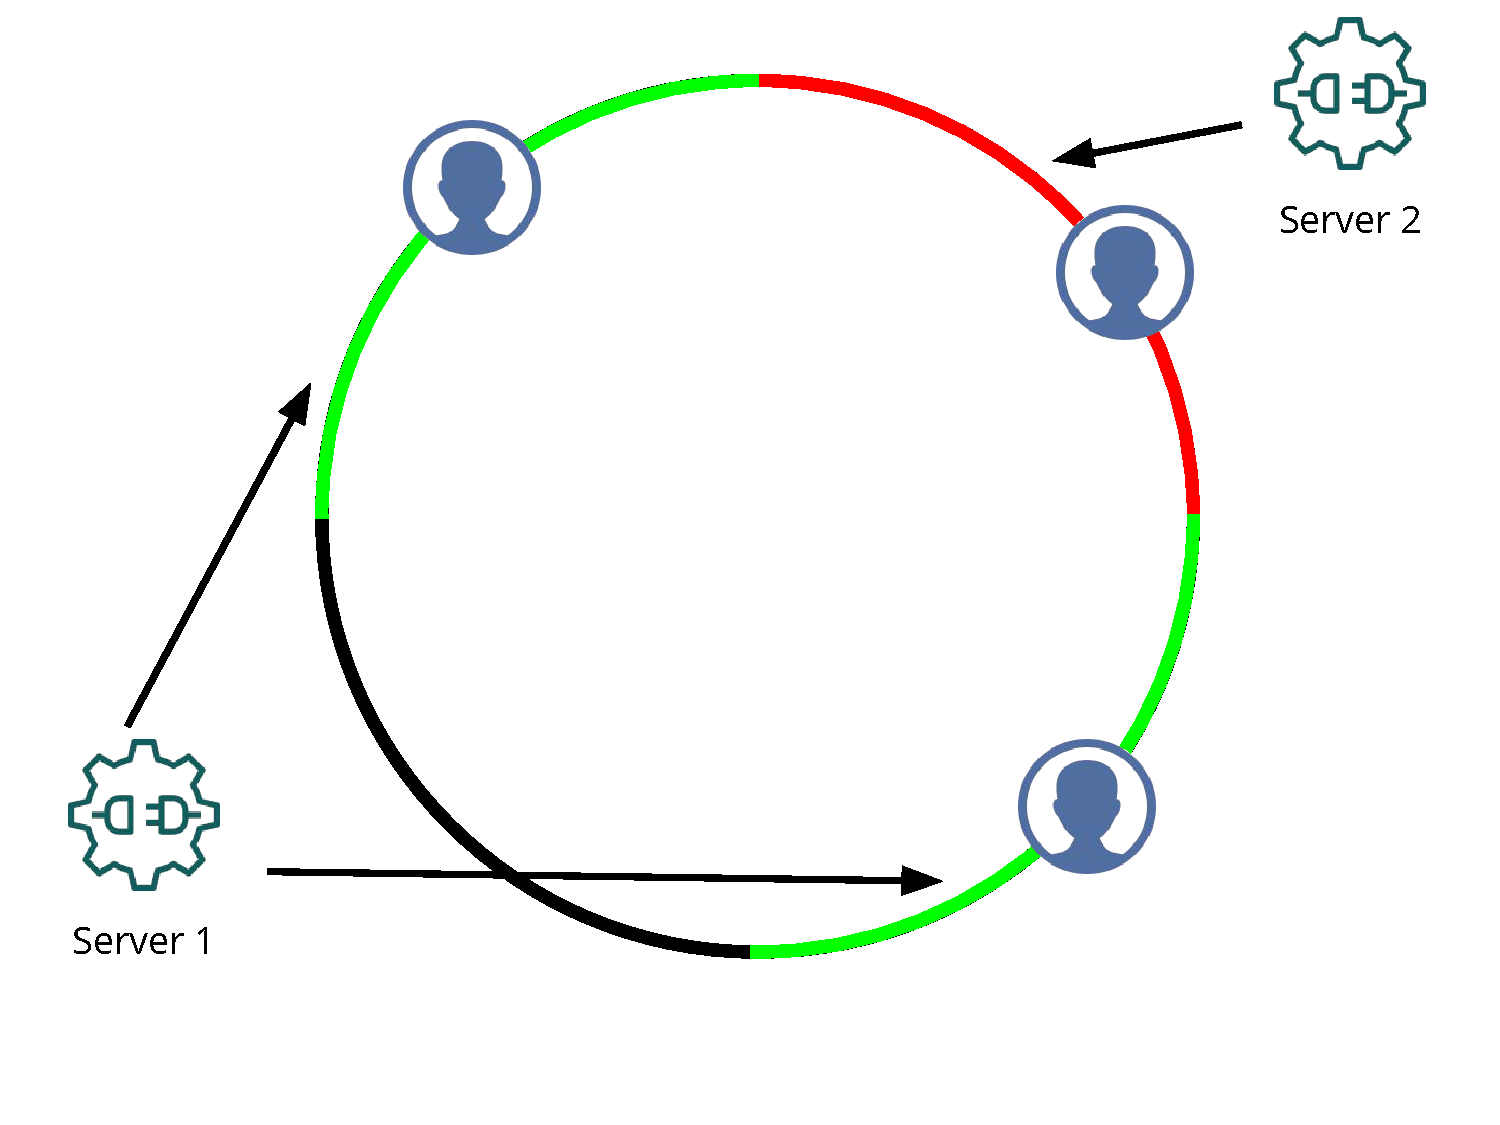
\includegraphics[width=0.6\linewidth]{figures/arch.pdf}
\caption{The Architecture of hDHT.}
\label{fig:arch}
\end{figure}

The architecture of hDHT is shown in Figure~\ref{fig:arch}.
In hDHT, the server control one or more contiguous segments on a \textit{consistent hashing ring}~\cite{}.
Each client has a position in the hashing ring which is determined based on the client physical location, using the \textit{Hilbert curve function}~\cite{}.
Each client thus \textit{registers} with the server that controls the segment containing the client.

In the example, Server 1 controls the two green segments, and stores the data for two clients.
Server 2 controls the red segment, and stores the data only of the client in that segment.
Other servers, not shown, control the rest the DHT curve.

\subsection{Client Interface}

Clients of hDHT are likely to be on a mobile device, as they should follow and record precisely the location of the user.
For this reason, our design moves most of the computation and networking to the server.

Each client is identified by a 160-bit node identifier.
This identifier is opaque to the client.
The client additionally stores its own position, as obtained from the GPS senstor, and the address of the server it is registered with.
The client interacts primarily with the registering server, but any time it can retrieve the address of the server responsible for any point in the curve.

Servers store simple client metadata, in the form of string key-value pairs.
Each server serves metadata requests only for the clients it is responsible for, which ensures consistency.

The full client-server interface is shown in Figure~\ref{fig:client-server}.

\begin{figure}
\small
\begin{itemize}
\item $\textsc{FindControllingServer}(\textit{node\_id}) \rightarrow \textit{address}$: find the address of the server controlling the given node ID; this request succeeds even if the node ID does not correspond to any client registered with the server
\item $\textsc{FindServerForPoint}(\textit{position}) \rightarrow \textit{address}$: find the address of the server controlling the given position
\item $\textsc{ClientHello}(\textit{position}, \textit{node\_id}) \rightarrow \textit{ok}, \textit{node\_id}$: register the client against this server; the client transmits both its own position and the previously obtained node ID, if available; the server responds \textit{Created} if the client was newly registered, \textit{AlreadyExists} if it recognized the previous node ID, or \textit{WrongServer} if the server is not responsible for the region of the Hilbert curve corresponding to \textit{position}.
\item $\textsc{Move}(\textit{position}) \rightarrow \textit{ok}, \textit{node\_id}, \textit{address}$: informs the server that the client moved; the server replies with the new node ID for the client, and either \textit{SameServer} or \textit{DifferentServer}, to indicate what server is now responsible for the client; if the client receives \textit{DifferentServer}, it must register with the new server
\item $\textsc{SetMetadata}(\textit{key}, \textit{value})$: set metadata for the calling client
\item $\textsc{GetMetadata}(\textit{node\_id}, \textit{key}) \rightarrow \textit{value}$: get metadata about the given client; the server forwards the request to the controlling server if needed
\end{itemize}
\caption{The hDHT client-server protocol}
\label{fig:client-server}
\end{figure}

\subsection{Hilbert Curves}

Client node IDs define the position of a client in the consistent hashing ring.
To facilitate location based queries, the node IDs are generated using a \textit{locality sensitive hash} that uses a Hilbert curve.

A Hilbert curve, or \textit{space-filling curve}, is a curve that passes all points in a grid exactly once and does not self intersect.
Hilbert curve can be constructed for grids of arbitrary dimension.
The Hilbert curve of order $k$, which covers the grid of size $2^k \times 2^k$, is constructed as a fractal, by refining the Hilbert curve of order $k-1$.
An efficient $O(k)$ algorithm exists to convert any point to the Hilbert curve to its coordinates in the grid and viceversa.

\subsection{Mapping Hilbert Curves to Consistent Hashing}

hDHT uses the Hilbert curve concept to generate the ID of the client.
First, the physical position of the client is mapped to a point in a rectangular Earth-sized grid.
Then, the point in the grid is converted to a point in the Hilbert curve, which provides the high bits of the node IDs.
The remaining low bits are assigned randomly.
This is a locality sensitive hashing because clients who are phyisically close will have similar Hilbert curve values, and thus will share some of the high bits of their node IDs.
Additionally, clients with similar high bits in the node IDs are more likely to be assigned to the same server, which improves the efficiency of serving requests.


\subsection{Serving Individual Requests}

\subsection{Routing with Incomplete Information}


Servers automatically move the metadata around during DHT rebalancing.
